%% Learning Cloth milestone report.
%% Adapted from the supplied Overleaf ACM sigconf template.
%% TeXCount configuration from the original template.
%TC:macro \cite [option:text,text]
%TC:macro \citep [option:text,text]
%TC:macro \citet [option:text,text]
%TC:envir table 0 1
%TC:envir table* 0 1
%TC:envir tabular [ignore] word
%TC:envir displaymath 0 word
%TC:envir math 0 word
%TC:envir comment 0 0

%% Use the original ACM proceedings class and its standard layout.
\documentclass[sigconf]{acmart}
\AtBeginDocument{\providecommand\BibTeX{{Bib\TeX}}}

%% Course submission metadata. This is not an ACM publication.
%% Replace these fields only if submitting to an actual conference.
\setcopyright{none}
\copyrightyear{2026}
\acmYear{2026}
\acmDOI{}
\acmISBN{}
\acmConference[CS 284A Milestone]{CS 284A Milestone Report}{November 22, 2026}{UC Berkeley}
\acmBooktitle{CS 284A Milestone Report, UC Berkeley, November 22, 2026}
\settopmatter{printacmref=true,printfolios=true}

%% SIGGRAPH uses author-year citations with the ACM bibliography style.
\citestyle{acmauthoryear}
\setlength{\emergencystretch}{2em}

%% Retain the standard reference block without claiming ACM publication.
\makeatletter
\patchcmd{\@mkbibcitation}{ACM, New York, NY, USA}{Course project report}{}{}
\makeatother

%% End of the preamble.
\begin{document}
%% Title and author information.
\title[Learning Cloth]{Learning Cloth: Evaluating Accuracy and Throughput of Physics Guided Residual Dynamics}
\subtitle{CS 284A Milestone Report | Progress as of November 22, 2026}
\author{Jimmy Wang}
\affiliation{%
  \institution{UC Berkeley}
  \city{Berkeley}
  \state{California}
  \country{USA}}
\email{jimmyhw@berkeley.edu}

\author{Charles Xu}
\affiliation{%
  \institution{UC Berkeley}
  \city{Berkeley}
  \state{California}
  \country{USA}}
\email{xuc@berkeley.edu}

\author{Jacob Ryan Lopez}
\affiliation{%
  \institution{UC Berkeley}
  \city{Berkeley}
  \state{California}
  \country{USA}}
\email{jacobrlopez22@berkeley.edu}

\author{Brian Chu}
\affiliation{%
  \institution{UC Berkeley}
  \city{Berkeley}
  \state{California}
  \country{USA}}
\email{bchu0@berkeley.edu}


\renewcommand{\shortauthors}{Wang et al.}
%% Abstract.
\begin{abstract}
We evaluate whether a learned residual improves cloth simulation accuracy and whether its cost is justified by GPU throughput. Our tabletop experiment compares a calibrated mass and spring model, Extended Position Based Dynamics (XPBD), and an adaptation of Physics Guided Residual Dynamics (PGRD). On eight synthetic test trajectories with an $8\times8$ cloth mesh, PGRD reduces motion RMSE from 1.95 mm to 1.76 mm, but increases final frame RMSE from 2.90 mm to 3.61 mm. On an Apple M5 Pro, fused Metal physics raises hybrid throughput to 28,700 environment steps per second at batch 64, about 1.8 times portable PyTorch MPS. The fused classical solvers remain substantially faster. These results show a modest improvement in average tracking error, but do not yet establish a speed advantage at matched accuracy or valid cloth contact. A separate MuJoCo experiment demonstrates a learned 3D world model for robot cloth manipulation, with visible prediction artifacts. We report progress on both experiments and identify the comparisons that remain.
\end{abstract}
%% CCS concepts and keywords replace the sample classification text.
\ccsdesc[500]{Computing methodologies~Physical simulation}
\ccsdesc[300]{Computing methodologies~Neural networks}
\ccsdesc[100]{Computer systems organization~Robotics}

\keywords{cloth simulation, residual dynamics, GPU computing, robotic manipulation}
%% Teaser figure, positioned by the ACM class before the body.
\begin{teaserfigure}
\centering
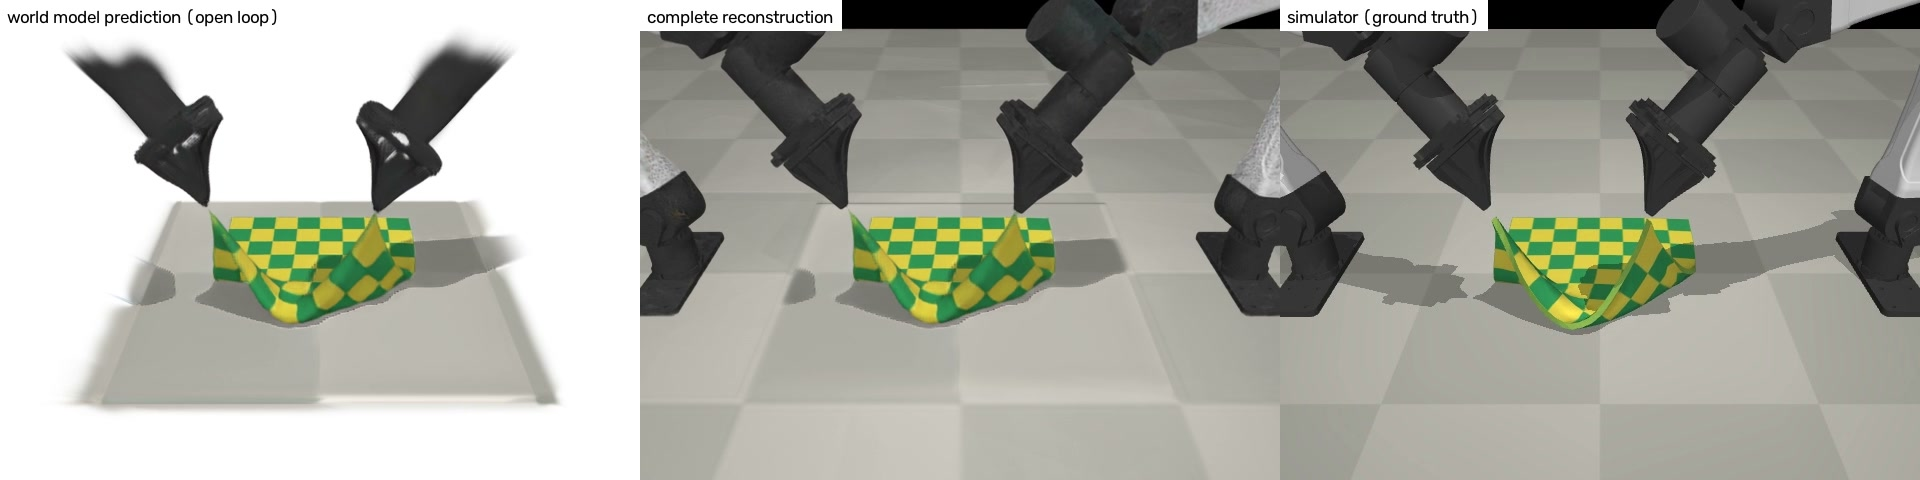
\includegraphics[width=\textwidth]{figures/robot-world-model.jpg}
\caption{Robot cloth manipulation shown in the milestone video. From left to right: open-loop world model prediction, complete reconstruction, and the MuJoCo simulator reference. This frame is taken at 7 seconds in the accompanying robot demonstration. The learned views reproduce the broad scene configuration but show visible artifacts, particularly around the robot arms. This experiment is separate from the PGRD accuracy and timing benchmark.}
\Description{Three views of two robot arms holding a green and yellow checkered cloth, comparing a predicted scene, a reconstructed scene, and the simulator.}
\label{fig:robot-world-model}
\end{teaserfigure}
%% Generate the title, authors, teaser, and standard ACM front matter.
\maketitle
\section{Introduction}

Robots can learn and practice tasks in simulation before attempting them on real hardware. For cloth folding, this depends on a simulator that captures how fabric stretches, bends, and makes contact with itself and the table. Matching a real cloth is difficult because its starting shape, material properties, and contact with the gripper may be uncertain.

Using smaller time steps can improve a simulation but also makes it slower. A learned model might approximate some of that detail at a lower cost, though its errors can accumulate over time. We study this tradeoff on a single cloth folding task using a calibrated spring solver, XPBD, and a spring solver with a learned residual correction. A learned model evaluated on these same benchmark trajectories remains future work. We also investigate a separate learned 3D world model of robot cloth manipulation. Our longer-term goal includes real-to-sim transfer from observed cloth data, but the results reported here use synthetic simulation data.

\section{Methods}

The first experiment separates two questions. 
Does the residual improve a calibrated spring rollout, and how much throughput does each method get on a GPU?

\subsection{Overview}

We have three runnable methods on the same 40 cm tabletop fold, an example PGRD checkpoint, and a reproducible synthetic test set. Two corners remain anchored while the opposite corners lift, cross the sheet, lower, and release. All solvers share the mesh, grasp trajectories, and 60 Hz control interval. XPBD follows the compliant constraint formulation of \citet{macklin2016xpbd}.

Our technical contribution is the tabletop adaptation of PGRD, a fused Metal implementation of the physics baselines, and a controlled evaluation that separates motion accuracy from execution cost. PGRD itself is prior work. We compare against a calibrated spring control to measure the additional effect of its learned residual. 

\subsection{Prior PGRD Work and Implementation}

Our hybrid follows Physics-Guided Residual Dynamics (PGRD)~\cite{patel2026pgrd}.

The paper first fits mass--spring parameters to trajectories, then trains a residual that sees the current state, previous state and spring prediction. The residual predicts a velocity change, which is added to the simulated velocity and integrated into a position change. Held vertices receive zero correction. The paper uses a Fourier-conditioned decoder, a gated temporal transformer and multi-step rollout training. It reports lower tracking error on a flag held by a supporting stick. 



Our fixed-mesh adaptation uses one-ring attention over triangle neighbors in place of Point Transformer V3. It has a smaller decoder and a two-layer, four-frame temporal transformer. A nine-point grid search fits spring stiffness and table friction. During training the five-step windows feed predictions back into the solver, with gradients through the residual network and its history. The spring step is frozen. We project the residual displacement against the table after it is applied, then update velocity consistently with that projection. The authors' separate release provides the original flag configuration and checkpoints~\cite{pgrdcode}. The upstream stack and its flag evaluation still need a Linux/CUDA run.


\subsection{Tools Used}
Table~\ref{tab:methods} identifies the implementations used in our comparison.

\begin{table}[!htbp]
  \caption{Overview of simulation methods and where to find them.}
  \label{tab:methods}
  \footnotesize
  \raggedright
  \begin{tabular}{@{}p{0.19\columnwidth} p{0.38\columnwidth} p{0.33\columnwidth}@{}}
    \toprule
    Method & What it does & Where to start \\
    \midrule
    Mass--spring &
      Semi-implicit Euler with stretch, shear and two-hop bending springs &
      \texttt{cloth\_\allowbreak sim.py}, \texttt{Torch\allowbreak Mass\allowbreak Spring} in \texttt{torch\_\allowbreak sim.py} \\
    XPBD &
      Compliant distance constraints with a sequential sweep over disjoint edge colors &
      \texttt{cloth\_\allowbreak sim.py}, \texttt{Torch\allowbreak XPBD} in \texttt{torch\_\allowbreak sim.py} \\
    PGRD &
      Calibrated spring step plus a learned velocity correction for each free vertex &
      \texttt{pgrd.py}, \texttt{train\_\allowbreak pgrd.py} \\
    Fused Metal physics &
      One GPU threadgroup per cloth, with all the physics substeps inside one dispatch per control step &
      \texttt{metal\_\allowbreak sim.py}, \texttt{cloth\_\allowbreak kernels.metal} \\
    Evaluation &
      Builds the fold, compares trajectories, and records latency and throughput &
      \texttt{benchmark.py}, \texttt{test\_\allowbreak simulation.py} \\
    \bottomrule
  \end{tabular}
\end{table}

\subsection{Held-Out Rollout Quality}

The demo uses an 8 $\times$ 8 mesh and 120 control steps. The generated folds vary lift height and timing. Seed 7 generates disjoint sets of 12 training, 4 validation and 8 test trajectories. The CPU teacher is XPBD with four substeps and twelve sweeps per substep. Calibration sees training folds. Checkpoint selection uses full validation rollouts. The demo checkpoint was selected at update 125 of 200 on the Apple M5 Pro.

\begin{table}[!htbp]
  \caption{Rollout and final-frame RMSE for each method.}
  \label{tab:rmse}
  \small
  \begin{tabular}{@{}lrr@{}}
    \toprule
    Method & Rollout RMSE & Final-frame RMSE \\
    \midrule
    Calibrated mass--spring & 1.95~mm & 2.90~mm \\
    PGRD & 1.76~mm & 3.61~mm \\
    \bottomrule
  \end{tabular}
\end{table}

The residual improves error over the full rollout by about 10\% and increases terminal error by about 24\%. The terminal result matters for a policy whose reward depends on the settled fold. The test data measures agreement with the XPBD teacher. This scene uses prescribed vertex grasps and a simple table plane. It omits cloth thickness and self-contact, so apparent layer alignment can occur even when the layers intersect. 

The \href{https://github.com/charlesxu0124/284A-final-project/blob/main/artifacts/training.json}{training record} contains the selected checkpoint and evaluation results.

We also trained with eight spring substeps using the same splits and validation rule. The hybrid reached 1.76 mm rollout and 3.37 mm final-frame RMSE, compared with 1.96 mm and 3.01 mm for its eight-substep spring control. With fused Metal at batch 64, the hybrids with eight and twelve substeps both ran at about 29k environment steps/s. Cutting four spring substeps made little difference once the spring computation was fused. The checkpoint is \texttt{pgrd-8substeps.pt} in the artifacts directory and uses the same reference file. 

The corresponding \href{https://github.com/charlesxu0124/284A-final-project/blob/main/artifacts/training-8substeps.json}{eight substep training record} is available separately.

\section{Results}

All timing results below were measured on an Apple M5 Pro.

Each environment has 64 vertices. Each control step advances the scene by 1/60 s. Mass--spring and the hybrid use 12 substeps. XPBD uses two substeps and four sweeps per substep. The calibrations, precision, folds and checkpoint are shared between the timing runs. CPU below means one PyTorch CPU thread. The GPU has two implementations. Portable PyTorch dispatches tensor operations individually. Fused Metal keeps each cloth's working positions in threadgroup memory and runs its physics in one kernel. PGRD's residual network still runs through PyTorch.

\begin{table*}[t]
  \caption{Single-cloth latency and batch-64 throughput for each solver.}
  \label{tab:performance}
  \small
  \setlength{\tabcolsep}{8pt}
  \centering
  \begin{tabular}{@{}lrrrrr@{}}
    \toprule
    & \multicolumn{2}{c}{Single-cloth median (ms)} & \multicolumn{3}{c}{Batch 64 (env steps/s)} \\
    \cmidrule(lr){2-3} \cmidrule(lr){4-6}
    Solver & CPU & Fused Metal & CPU & PyTorch MPS & Fused Metal \\
    \midrule
    Mass--spring & 0.52 & 0.20 & 13.6k & 33.9k & 1.39M \\
    XPBD & 1.06 & 0.21 & 18.4k & 11.2k & 1.19M \\
    PGRD & 0.84 & 0.92 & 4.33k & 15.9k & 28.7k \\
    \bottomrule
  \end{tabular}%
\end{table*}

The fused classical solvers are much faster on this small scene. At batch 64, fusion improves hybrid throughput about 1.8$\times$ over PyTorch MPS and 6.6$\times$ over one CPU thread. PGRD still takes far more compute than either fused physics baseline. Portable XPBD illustrates why GPU placement by itself can be slow. Each sequential edge color incurs a group of dispatches, so small batches can be dominated by launch overhead.

Latency synchronizes after every control step. Throughput synchronizes after blocks of 16 steps, keeping state and prescribed actions resident on the selected device. Warm-up, trajectory recording, CPU transfers for metrics and disk I/O are outside the timed region. The numbers cover cloth dynamics, prescribed grasps and table contact. They exclude policy inference, observation rendering and robot dynamics. The profile includes medians, p95s and batches of 1, 16, 64 and 256. It also includes a batch-256 CPU run with four PyTorch threads. These are single-machine measurements. 

The complete \href{https://github.com/charlesxu0124/284A-final-project/blob/main/artifacts/profile-m5-pro.json}{timing profile} is available with the code.


\begin{figure*}[t]
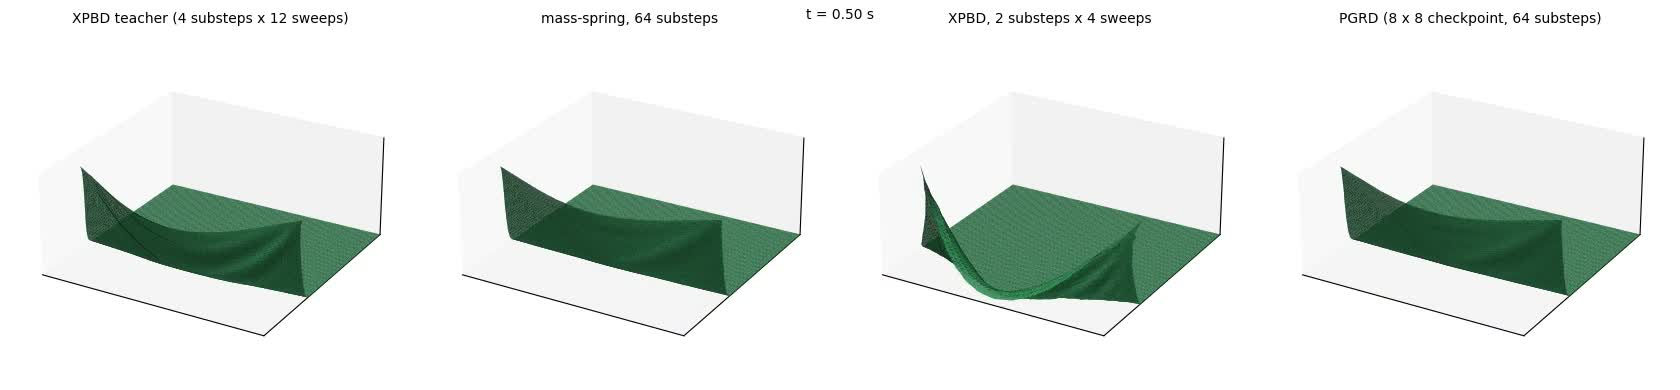
\includegraphics[width=\textwidth]{figures/solver-comparison.jpg}
\caption{Additional visualization at $64\times64$ resolution: XPBD teacher, spring model, XPBD baseline, and PGRD from left to right. The video labels the PGRD model as an $8\times8$ checkpoint applied with 64 spring substeps. These settings differ from the $8\times8$ accuracy and timing experiments, so this figure illustrates behavior rather than supplying evidence for the tabulated measurements.}
\Description{Four cloth meshes compared at the same time during a fold.}
\end{figure*}

\section{Robot Cloth Manipulation and Learned World Model}
As a second part of our milestone, we implemented a MuJoCo scene with two robot arms manipulating cloth and used the \href{https://github.com/jwang771/3d-world-simulator}{3D World Simulator} to learn its visual dynamics. The project pipeline renders each episode from four cameras. An autoencoder maps these views to a voxel latent representation that decodes to Gaussian scene representations. A dynamics model predicts the next latent from recent latent states and robot actions. This experiment uses MuJoCo flex cloth rather than the spring or XPBD cloth in the numerical benchmark~\cite{projectcode}.

Figure~\ref{fig:robot-world-model} shows a frame from the robot demonstration included in our narrated milestone video. The left panel is the world model prediction in an open-loop rollout, the center panel is the complete reconstruction, and the right panel is the simulator reference. The model captures the broad cloth configuration and robot motion, but visible artifacts remain around the arms and scene geometry. This is a qualitative progress result. We have not reported a matched accuracy or throughput comparison between this learned world model and the classical solvers.

The demonstration shows cloth holding and movement, rather than a completed folding task. Our next steps are to measure the cost and quality of the neural simulation and to investigate contact and robot interaction in the classical cloth implementations. Real-to-sim transfer remains a research goal, not a result established by these synthetic sequences.

\begin{figure*}[t]
\centering
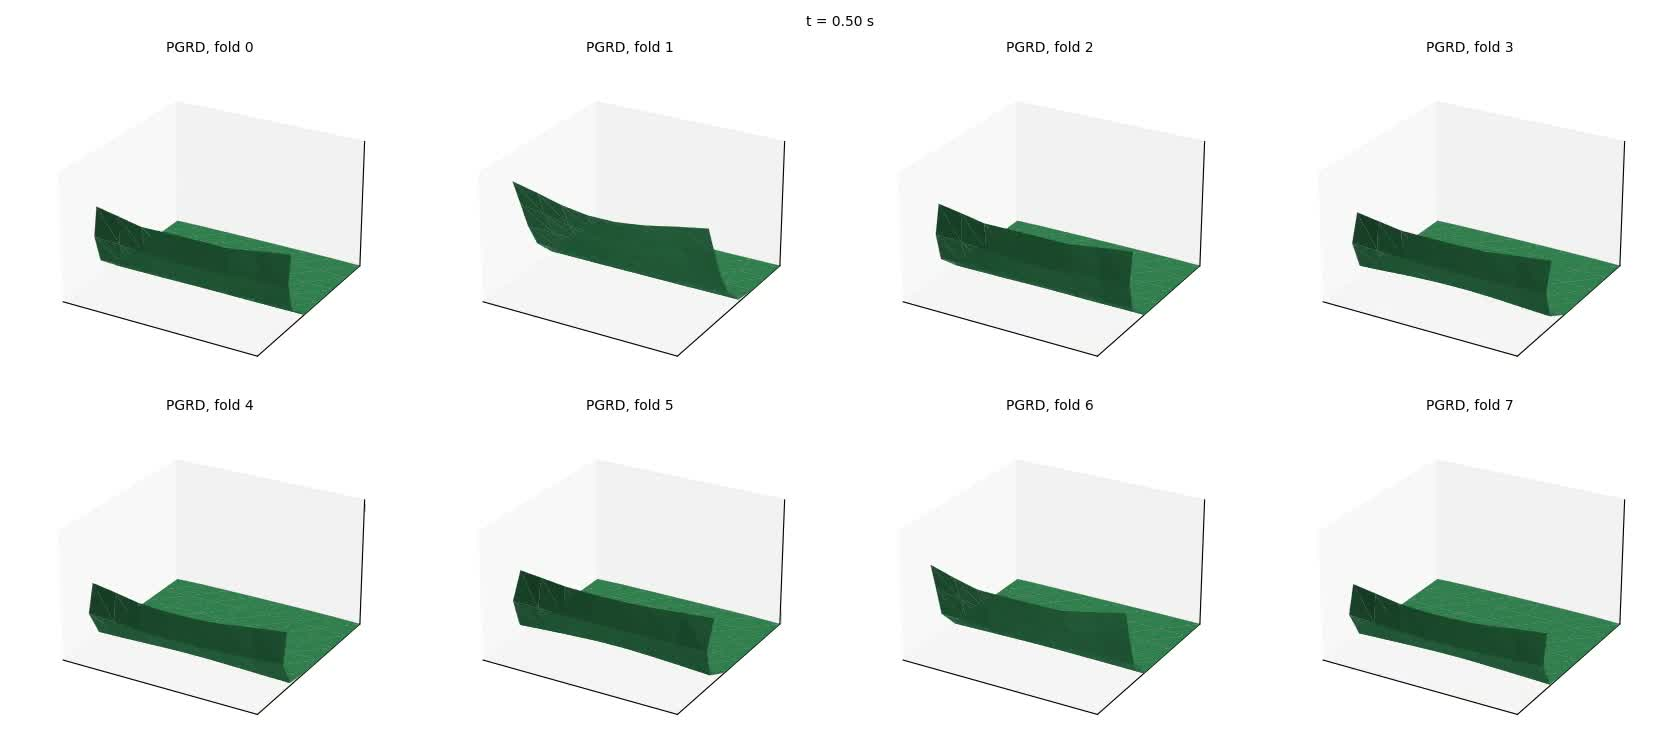
\includegraphics[width=0.85\textwidth]{figures/test-folds.jpg}
\caption{Eight test folds predicted by the project PGRD model. The views show different grasp trajectories at the same simulation time. The experiment evaluates numerical agreement with an XPBD teacher and does not include cloth self contact.}
\Description{Eight green cloth meshes undergoing tabletop folds, arranged in two rows of four.}
\end{figure*}

\section{Discussion and Limitations}
\subsection{Average accuracy and final fold quality}
The residual improves error averaged over the sequence, but the terminal result moves in the opposite direction. For robotic folding, these objectives need to be evaluated separately. A lower mean error does not imply a more accurate settled fold. The additional experiment with eight spring substeps shows the same pattern, which suggests that reducing the physics budget alone does not resolve the terminal error in the current setup. We have not measured statistical significance across independent training runs, so the reported differences should be treated as preliminary measurements of the supplied checkpoints.

The reference trajectories come from XPBD rather than captured cloth motion. Consequently, the experiment measures how well a model approximates this teacher. It does not establish material fidelity or transfer to real cloth. The teacher uses a larger solver budget than the timed XPBD baseline, so those two XPBD configurations serve different purposes. The teacher provides reference motion, while the baseline provides a cheaper physics comparison.

\subsection{Execution cost and hardware}
The hybrid benefits from kernel fusion, but its residual network still requires separate PyTorch computation. Reducing the number of spring substeps from twelve to eight has little effect on throughput after fusion. This is consistent with the remaining cost being dominated by work outside the fused spring step, although component profiling is needed to attribute that cost precisely.

A single cloth and a batch of cloths also answer different performance questions. PGRD has higher single cloth latency on fused Metal than on one CPU thread in this experiment, even though batching improves GPU throughput. A planning system with sequential dependencies may care about latency, whereas a system collecting many independent trajectories may benefit from throughput. Neither measurement includes policy evaluation or visual observations.

The results are specific to one machine, a small cloth, and the reported solver budgets. They do not establish a general ranking across hardware or mesh resolutions. CUDA support is present in the portable implementation but has not yet been verified in the reported experiments. In particular, moving a sequence of small tensor operations to a GPU does not automatically make it faster.

\subsection{Contact and scope}
The current tabletop scene includes prescribed vertex grasps and plane contact, but omits cloth thickness, self contact, and robot dynamics. A visually plausible fold may therefore contain intersecting layers. This limitation affects both the interpretation of tracking error and the practical value of the final configuration. Future evaluation should include contact violations and a settled fold score alongside vertex error.

The separate robot experiment includes simulated arms, but it does not extend the tabletop PGRD benchmark with robot contact. Its cloth representation and prediction outputs differ from those of the solver comparison, so the two experiments are not yet a controlled comparison.

\section{Reproducibility}
The code, checkpoints, synthetic reference trajectories, training records, and timing profile are available in the project repository~\cite{projectcode}. The reported accuracy run uses resolution 8, batch 8, the test split, and seed 7 with \path{artifacts/test-reference.npz}. The benchmark checks that the reference matches the mesh, action schedule, and time step. Both motion and final frame RMSE exclude vertices held during the measured frame. This prevents prescribed grasp positions from artificially lowering the error.

For batch scaling, the generator preserves the first eight test trajectories and adds trajectories from the same generator. Output files contain solver trajectories and JSON measurements. Trajectories store positions in meters with frame, environment, vertex, and coordinate dimensions, together with rest geometry and the action schedule. Keeping the checkpoint, precision, mesh, and inputs fixed makes backend comparisons easier to interpret.

The repository test suite checks agreement between CPU implementations, verifies that a zero residual recovers the spring model, and checks that training, validation, and test trajectories are distinct. On supported Apple hardware it also compares PyTorch MPS and fused Metal against PyTorch CPU. These checks establish implementation consistency within their tested settings. They do not validate the material model against real cloth.



\section{Next Experiments}
We will retain PGRD and its fitted spring control, add Newton VBD as another GPU physics baseline, and train a MeshGraphNets style learned dynamics control on the same trajectories~\cite{newton,pfaff2021mesh}. The goal is to sweep solver budgets and compare throughput at matched motion error and contact quality. This will test whether learning provides a useful computational tradeoff rather than simply improving one accuracy measure.

A teacher with more complete contact handling, such as C-IPC, would allow experiments that account for cloth layer separation~\cite{cipc}. We plan to measure error over different prediction horizons, self intersections, and final fold quality. Validation against observed cloth motion could use the cloth manipulation benchmark of \citet{blanco2024benchmark}. These experiments remain future work.

We also plan to verify the portable CUDA path and the original PGRD flag evaluation on Linux and NVIDIA hardware. Cross hardware comparisons should use the same checkpoint, precision, resolution, and batch sizes before introducing backend specific optimizations. Larger meshes may require more spring substeps, which must be reported rather than silently changed.

\section{Conclusion}
Our current experiment demonstrates a tabletop residual model and a reproducible comparison of accuracy and GPU execution cost. PGRD lowers average error against an XPBD teacher by about 10\%, but its final frame error is worse. Fused physics improves hybrid throughput while leaving the classical solvers much faster on the tested small scene. The evidence therefore supports a limited accuracy benefit, not a general speed advantage for learning. The separate robot experiment demonstrates learned scene prediction with visible artifacts. Matching error and contact quality across solver budgets, and evaluating robot interaction, are the next steps toward a broader comparison.

\section*{Project Materials}
\noindent\textbf{Milestone video:} \href{https://jacobrlopez.github.io/cs284a-project/assets/videos/cs284-milestone-video.mp4}{Watch the narrated progress update}.\par
\noindent\textbf{Presentation slides:} \href{https://docs.google.com/presentation/d/10qQ5zAVu4HsRSvfzTfzSnumnGHDP_jmQl_tjDnVh7NU/edit}{View the milestone slides}.\par
\noindent\textbf{Project webpage:} \href{https://jacobrlopez.github.io/cs284a-project/}{Read the project summary and view demonstrations}.\par
\noindent\textbf{Code:} \href{https://github.com/charlesxu0124/284A-final-project}{Source code and experiment artifacts}.\par
The video presents both the solver comparison and the robot world model demonstration. The earlier \href{https://drive.google.com/file/d/1KOEwjS67DSdJb9yQWuCjANsEz6WcbaMj/view}{voice recording} is also available. These materials document current progress.

\section*{Author Contributions}
\textit{To be completed by the authors before submission.}
% Add the specific contributions of Jimmy Wang, Charles Xu,
% Jacob Ryan Lopez, and Brian Chu here.
%% References use the original template bibliography style.
\bibliographystyle{ACM-Reference-Format}
\bibliography{references}
%% Optional template elements are retained as comments, not sample prose.
%% Add acknowledgments here only when there are actual people or support to credit.
% \begin{acks}
% \end{acks}
%% Add an appendix here only when supplemental material is needed.
% \appendix
% \section{Supplemental Results}

\end{document}
\endinput
